\documentclass{ieeeaccess}
\usepackage{cite}
\usepackage{graphicx}
\usepackage{amsmath,amssymb,amsfonts}

% ieeeaccess.cls (third-party mirror) uses the counter "biography" and the flag
% "@biographyTOCentrynotmade" inside the biographynophoto environment without
% ever declaring them -- declare manually here to avoid compile errors.
\newcounter{biography}
\makeatletter
\newif\if@biographyTOCentrynotmade
\@biographyTOCentrynotmadetrue
\makeatother

% \@makecaption in this class compares \xfigwd (figure width) against
% \columnwidth to pick a caption style, but \xfigwd is only ever set by the
% class's own \Figure macro -- not used here (plain figure/figure* is used
% instead). Declare it here and ALWAYS set it to 0pt right before each
% \caption (\ifdim 0pt>\columnwidth is always FALSE), which selects the
% short-caption branch: plain \raggedright text that wraps at whatever
% \hsize is in effect (\textwidth inside figure*, \columnwidth inside
% figure), so it always wraps correctly. Do NOT use the "wide" branch
% (\xfigwd=\linewidth/\textwidth): it renders the caption as a single-line
% tabular with no width constraint, so it does NOT wrap -- a long caption
% silently overflows past the page margin with no error (only visible as
% an "Overfull \hbox" warning in the log).
\newdimen\xfigwd

\begin{document}

\doi{10.1109/ACCESS.2017.DOI}

\title{Graph Retrieval-Augmented Generation for Improving Retrieval Precision and Syntactic Validity in Kubernetes Configuration}

\author{\uppercase{Jihan Aurelia}\authorrefmark{1}, \uppercase{Dimitri Mahayana}\authorrefmark{1}, and \uppercase{Naufal Irsyadi}\authorrefmark{1}}
\address[1]{School of Electrical Engineering and Informatics, Institut Teknologi Bandung, Bandung 40132, Indonesia}

\markboth
{Aurelia \headeretal: GraphRAG for Kubernetes Configuration}
{Aurelia \headeretal: GraphRAG for Kubernetes Configuration}

\corresp{Corresponding author: Jihan Aurelia (e-mail: 18222001@std.stei.itb.ac.id).}

\begin{abstract}
Kubernetes has become the de facto standard for container orchestration, yet the complexity of its YAML configuration drives the use of Large Language Models (LLMs) that are prone to producing semantically incorrect configurations. Vector-based retrieval-augmented generation (RAG) is insufficient because it fails to capture the hierarchical relations among Kubernetes components. This work builds a graph retrieval-augmented generation (GraphRAG) system that derives a knowledge graph (KG) deterministically from the Kubernetes OpenAPI specification, traverses it with a depth that adapts to query intent, and validates generated YAML manifests directly against the graph without requiring a live cluster. The system is evaluated against Vector RAG and a context-free LLM using 102 practitioner-validated test scenarios. Results show a clear advantage on the retrieval dimension: an F1 score of 0.71 versus 0.24 for Vector RAG, a statistically significant difference (p$<$0.001). Graph traversal also successfully covers most of the expected schema relations, reaching a hop accuracy of 0.76. In contrast, answer text quality does not differ significantly across systems, indicating that the knowledge graph's contribution lies in the traceability and completeness of structural retrieval rather than in language fluency. These findings empirically map the dimensions where graph representation provides a genuine advantage in the Kubernetes configuration domain.
\end{abstract}

\begin{keywords}
graph retrieval-augmented generation, intent-adaptive depth traversal, knowledge graph, Kubernetes, LLM hallucination, YAML validation
\end{keywords}

\titlepgskip=-15pt

\maketitle

\section{Introduction}
\label{sec:pendahuluan}

\PARstart{K}{ubernetes} \cite{k8s_docs_concepts} has established itself as the de facto industry standard for container orchestration, driven by a mature ecosystem and the flexibility of declarative infrastructure management \cite{cncf_2023_survey,gartner_cloud_2021}. However, this declarative paradigm requires developers to write verbose, hierarchical YAML configurations with strong inter-object dependencies that are frequently left implicit \cite{soldani_pains_2018}. As a consequence of this complexity, roughly 80\% of Kubernetes operational incidents are rooted in this configuration complexity, and 18\% of open-source configuration files have been found to contain serious security vulnerabilities \cite{rahman2023misconfigurations}.

This situation has driven the use of LLMs to help compose and explain Kubernetes configurations. However, LLMs can generate code that appears syntactically correct yet is semantically wrong \cite{liu2024deepanalysis}, a common manifestation of the broader hallucination tendency of generative models \cite{ji_hallucination_2023}. Mitigation efforts through vector-based retrieval-augmented generation (RAG) also fall short: such approaches rely solely on embedding similarity and therefore fail to capture the causal and hierarchical relations that form the core logic of the Kubernetes domain \cite{wan2025empowering}.

The graph retrieval-augmented generation (GraphRAG) literature addresses part of this limitation by injecting structured knowledge representations into the retrieval process \cite{han_graphrag_2024}. However, as detailed in \S\ref{sec:related}, two technical gaps persist: existing knowledge-graph construction pipelines are largely LLM-driven and therefore difficult to reproduce across runs, and existing traversal mechanisms typically apply a fixed depth uniformly across all query types despite markedly different context needs.

Based on these two gaps, this work proposes three technical contributions. First, a deterministic knowledge-graph construction pipeline based on the OpenAPI schema, so that extraction results are consistent across runs. Second, a traversal mechanism whose depth adapts to the query intent type (intent-adaptive depth traversal), rather than a uniform fixed depth. Third, a three-layer, KG-grounded structural YAML validation mechanism that serves as a static alternative to a dry-run against a live Kubernetes cluster. The remainder of this paper reviews related work (\S\ref{sec:related}), presents the system design (\S\ref{sec:perancangan}), describes the evaluation setup (\S\ref{sec:evaluasi}), reports results and discussion (\S\ref{sec:hasil}), and concludes (\S\ref{sec:kesimpulan}).

\section{Related Work}
\label{sec:related}

\subsection{RAG and LLM Hallucination in Technical Domains}

Retrieval-augmented generation (RAG) has become a standard approach for grounding LLM output in external knowledge, reducing hallucination by conditioning generation on retrieved context \cite{rag_survey}. RAG pipelines built on generic chunking and vector similarity nevertheless remain vulnerable to weak semantic boundaries between retrieved passages, which has motivated chunking strategies that better align retrieval units with document structure \cite{moreno2025rag}. Evaluation frameworks such as RAGAS \cite{es_ragas_2023} formalize this concern by decomposing answer quality into sub-metrics, including faithfulness (the traceability of generated claims to retrieved context) and answer relevance, both of which this work adopts (\S\ref{sec:evaluasi}). Hallucination itself remains an open problem for generative models in general \cite{ji_hallucination_2023}, and is particularly consequential for code and configuration generation, where syntactically plausible output can still be semantically wrong \cite{liu2024deepanalysis}. Together, these findings motivate retrieval mechanisms with an explicit, inspectable structure rather than opaque similarity search alone.

\subsection{Knowledge Graph Construction: LLM-Based vs.\ Schema-Derived}

Constructing the knowledge graph itself is an open research question. A substantial body of work uses an LLM to extract entities and relations directly from unstructured text \cite{pan2024unifying,ma_llm_kg_2025}, and surveys of graph construction techniques document a wide range of such extraction pipelines \cite{hofer2024construction}. Because LLM-based extraction is inherently stochastic, however, the resulting graph structure varies across runs, which complicates reproducibility and auditability, a concern also raised more broadly in domain-specific knowledge-graph construction \cite{abusalih2021domain}. Schema-derived construction, in which a graph is built by explicit, deterministic transformation rules applied to a formal specification rather than by model inference, offers an alternative that avoids this variability, but it has received comparatively little attention for API-defined domains such as Kubernetes.

\subsection{GraphRAG and Traversal Strategies}

GraphRAG systems combine graph traversal with LLM generation to answer questions grounded in structured knowledge. G-Retriever \cite{he2024gretriever} retrieves relevant subgraphs for textual graph question answering; HSG-RAG \cite{hsgrag2025acm} constructs a hierarchical knowledge base for embedded system development; a GraphRAG-enhanced dialogue engine has been applied to a civil IoT platform \cite{civiot2025graphrag}; and NeuSym-RAG \cite{cao2025neusymrag} combines neural and symbolic retrieval for structured document question answering. Across these systems, graph traversal typically proceeds to a fixed depth regardless of query type, an assumption inherited from general-purpose GraphRAG formulations \cite{han_graphrag_2024}. Applied specifically to Kubernetes documentation, hybrid retrieval-augmented generation has been shown to outperform purely vector-based retrieval by incorporating structured domain knowledge \cite{wan2025empowering}, but without varying traversal depth by query intent and without validating generated output against the graph itself. This work addresses both gaps directly.

\section{System Design}
\label{sec:perancangan}

Fig.~\ref{fig:arsitektur} summarizes the architecture of the GraphRAG system, spanning an offline knowledge-graph construction zone and a runtime retrieval-and-generation zone.

\begin{figure*}[t]
    \centering
    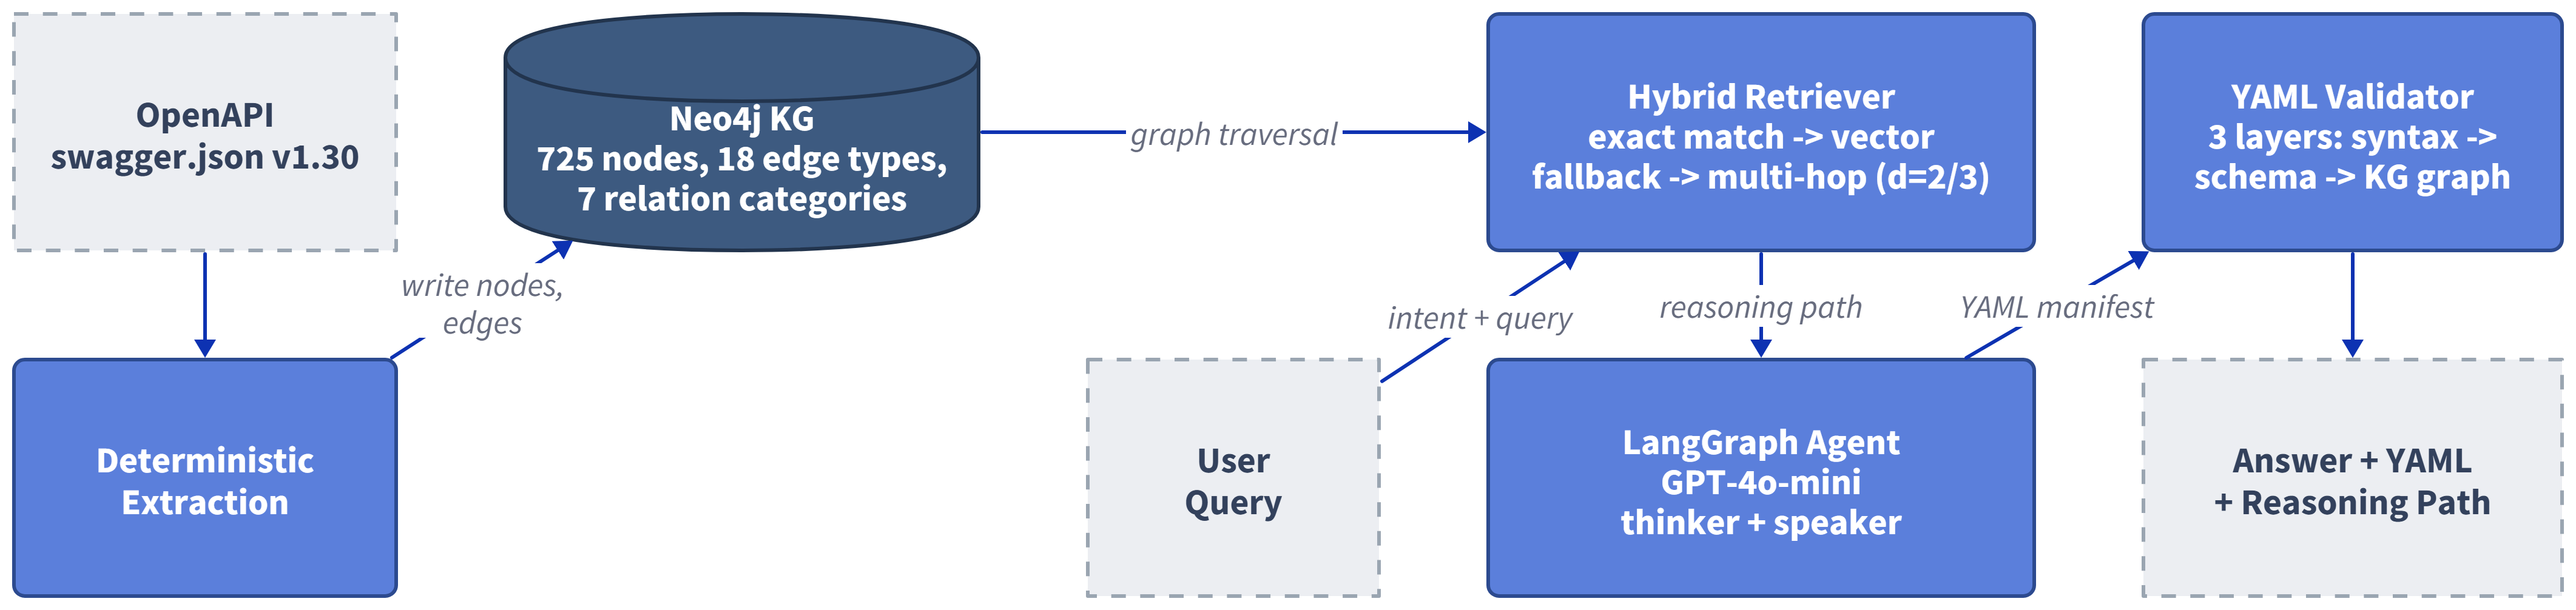
\includegraphics[width=0.92\textwidth]{figures/en/fig1_architecture.png}
    \xfigwd=0pt
    \caption{GraphRAG system architecture: deterministic knowledge-graph construction from \texttt{swagger.json} (left), and the retrieval and answer-generation flow with graph-grounded YAML validation (right).}
    \label{fig:arsitektur}
\end{figure*}

\subsection{Deterministic Knowledge Graph Construction}

The knowledge graph is built directly from the \textit{definitions} block of the Kubernetes OpenAPI specification (\texttt{swagger.json}) through explicit transformation rules, yielding 725 nodes and 18 edge types across 7 semantic relation categories (structural, workload, storage, configuration, networking, RBAC, and autoscaling). Graph construction uses two complementary strategies: a deterministic strategy that converts every \texttt{\$ref}, \texttt{allOf}, \texttt{oneOf}, and \texttt{anyOf} reference directly into a structural edge, and a semi-deterministic strategy that forms domain-relevant operational relations that are not explicitly stated in the schema, such as the relation between \textit{Service} and \textit{Pod}. Because every transformation rule is explicit and executed without any stochastic component, the resulting graph is consistent across runs and every edge can be traced back to its originating schema reference, unlike LLM-based extraction approaches. The semantic vector representation of each node is stored directly as a graph property in Neo4j, so similarity-based search can be executed within the same graph without a separate vector store.

\subsection{Retrieval with Adaptive Depth}

The retriever module implements a three-stage cascading retrieval process. The first stage searches for a node whose name exactly matches the entity extracted from the query intent and uses it as the seed node; this gives the highest precision because it relies on exact matching rather than semantic approximation. The second stage, executed only if the first stage fails, searches for the node with the highest vector similarity to the query as a fallback. The third stage recursively traverses the graph from the seed node with a depth limit that adapts to the query intent type: a depth of 2 for the \textit{explain} and \textit{followup} intents, which are resource-specific, and a depth of 3 for the \textit{generate\_yaml}, \textit{trace\_relationship}, and \textit{planning} intents, which require broader relational context. This bound was chosen because nodes beyond depth 3 are dominated by generic types shared by dozens to hundreds of resources, which lowers context precision without adding relevant information. The relational path traversed is assembled into a reasoning path and injected into the prompt as verifiable evidence for the user.

\subsection{Three-Layer Knowledge-Graph-Grounded YAML Validation}

When a query's intent is classified as \textit{generate\_yaml}, the resulting YAML manifest passes through three sequential validation layers: the first layer checks syntactic correctness using a standard YAML parser; the second layer checks structural compliance against the official Kubernetes schema; and the third layer queries the knowledge graph directly to verify that all required fields are present for each resource. This third layer is what makes the validation KG-grounded: required-field verification is performed without needing a dry-run against a live Kubernetes cluster, because the same schema information is already available in the graph built during construction.

All of the above mechanisms run on a LangGraph pipeline in which GPT-4o-mini plays a dual role as \textit{thinker} (intent classification and entity extraction) and \textit{speaker} (answer generation), with Neo4j serving as both graph storage and a unified vector index, and a lightweight database providing session-based conversational memory.

\section{Evaluation Setup}
\label{sec:evaluasi}

Evaluation uses 102 test scenarios (fixtures) spread across eight question categories: \textit{conceptual} (25), \textit{yaml\_gen} (25), \textit{relationship} (18), \textit{followup} (12), \textit{realworld} (9), \textit{planning} (5), \textit{troubleshooting} (5), and \textit{command} (3). These scenarios were constructed from interviews with three DevOps/SRE practitioners who actively use Kubernetes and LLMs. The three practitioners also rated the realism of sample fixtures, confirming that scenarios grounded in concrete operational situations were judged more representative than purely definitional questions.

System performance is measured along three dimensions. \textit{Answer Quality} (AnsQ) is the average of the answer's semantic similarity to the ground truth, YAML syntactic validity, and schema compliance. \textit{Retrieval Quality} (RetQ) is operationalized as an F1 score between the set of nodes on the system's reasoning path and the set of relevant ground-truth nodes, following the standard Precision/Recall definitions \cite{manning_ir_2008}:
\begin{equation}
\text{RetQ}_{F1} = \frac{2 \cdot P \cdot R}{P + R}
\label{eq:f1}
\end{equation}
where $P$ and $R$ denote the Precision and Recall of the reasoning-path nodes against the relevant ground-truth nodes, respectively. \textit{Reasoning Quality} (ReaQ) has two components: \textit{hop accuracy}, the proportion of ground-truth edges successfully traversed by the system,
\begin{equation}
\text{HopAcc} = \frac{|E_{\text{traversed}} \cap E_{\text{ground truth}}|}{|E_{\text{ground truth}}|},
\label{eq:hopacc}
\end{equation}
and \textit{faithfulness}, the proportion of answer claims that can be traced back to the retrieved context \cite{es_ragas_2023}.

These three dimensions are measured to compare three systems using the same dataset, the same speaker model (GPT-4o-mini, temperature=0.1), and identical metrics: \textit{Vanilla LLM} (no context), \textit{Vector RAG} (cosine-similarity top-5 without graph traversal), and GraphRAG (the full system). Statistical significance is tested using the Wilcoxon signed-rank test with a paired bootstrap of 1,000 iterations and Holm-Bonferroni correction for multiple comparisons.

In addition to these quantitative metrics, four independent Kubernetes practitioners rated GraphRAG's answers on three representative scenarios (YAML manifest generation, troubleshooting a failing Pod, and explaining a resource relationship) on a 1--5 scale covering relevance, technical accuracy, completeness, and willingness to use the answer in practice. The system's retrieval trace received the highest average confidence rating among all rated items (4.50 out of 5), and the relationship-explanation scenario received the highest average score across all four dimensions (4.38). This qualitative check complements, rather than replaces, the quantitative evaluation; its purpose is to confirm that the automated metrics track something practitioners actually value.

\section{Results and Discussion}
\label{sec:hasil}

\subsection{Three-System Comparison}

Table~\ref{tbl:perbandingan} summarizes the three systems' scores across all evaluation dimensions together with their statistical significance. RetQ is the most discriminative dimension: GraphRAG reaches an F1 of 0.71 versus 0.24 for Vector RAG and 0.00 for Vanilla LLM, both differences significant (p$<$0.001). This advantage stems from multi-hop traversal reaching intermediate structural nodes (e.g., the \textit{Deployment}~$\to$~\textit{DeploymentSpec}~$\to$~\textit{PodTemplateSpec} chain) that Vector RAG cannot access. In contrast, AnsQ is comparable across all three systems, and the difference between GraphRAG and Vector RAG is not statistically significant ($p_{\text{Holm}}=0.067$), indicating that answer text quality is determined by the generative capability of the LLM, which is identical across all three systems, rather than by the retrieval mechanism.

\begin{table*}[t]
\caption{Three-System Score Comparison per Evaluation Dimension ($n=102$)}
\label{tbl:perbandingan}
\centering
\begin{tabular}{|l|c|c|c|c|c|}
\hline
\textbf{Metric} & \textbf{Vanilla LLM} & \textbf{Vector RAG} & \textbf{GraphRAG} & \textbf{$\Delta$ vs.\ Vector RAG} & \textbf{$\Delta$ vs.\ Vanilla LLM} \\
\hline
AnsQ & 0.7469 & 0.7984 & 0.8031 & $+0.005$ (n.s.) & $+0.056$ (***) \\
\hline
RetQ (F1) & N/A & 0.2437 & 0.7089 & $+0.465$ (***) & $+0.709$ (***) \\
\hline
Hop Accuracy & N/A & N/A & 0.7562 & N/A & N/A \\
\hline
Faithfulness & N/A & 0.1675 & 0.3055 & $+0.127$ (***) & N/A \\
\hline
Syntactic Validity & 0.8333 & 0.9333 & 1.0000 & $+0.036$ (n.s.) & $+0.143$ (*) \\
\hline
\end{tabular}
\\[4pt]
{\footnotesize \raggedright N/A = not applicable or not computable (no retrieval or graph traversal for that system/metric pairing). *** $p<0.001$; * $p<0.05$; n.s.\ = not significant (Wilcoxon + paired bootstrap, 1{,}000 iterations, Holm-Bonferroni correction).\par}
\end{table*}


\subsection{Component Contributions}

Table~\ref{tbl:ablasi} presents the results of a seven-configuration ablation study, while Fig.~\ref{fig:ablasi} visualizes the most notable drops in RetQ and hop accuracy. Disabling multi-hop traversal (A2) produces the largest RetQ drop, confirming that this component is the most critical: without traversal, the system obtains only the seed node and lacks the schema-dependency context. Disabling exact match (A1) also significantly lowers RetQ, confirming this stage's role as the gate that ensures seed-node accuracy. Replacing 18 semantic edge types with a single generic type (A7) significantly lowers both RetQ and hop accuracy, demonstrating the relation taxonomy's contribution to retrieval and reasoning quality. In contrast, a fixed depth of $d=3$ (A4) does not significantly lower RetQ but does increase hop accuracy, showing that adaptive behavior cannot be fully replaced by a single fixed depth: greater depth increases the coverage of traversed edges but lowers RetQ precision because it draws in additional, less-relevant nodes.

\begin{table}[t]
\caption{Ablation Study: Difference from the GraphRAG Baseline ($n=102$)}
\label{tbl:ablasi}
\centering
\begin{footnotesize}
\begin{tabular}{|p{0.36\linewidth}|c|c|c|}
\hline
\textbf{Configuration} & \textbf{$\Delta$AnsQ} & \textbf{$\Delta$RetQ} & \textbf{$\Delta$HopAcc} \\
\hline
A1 \textit{no\_exact\_match} & $-0.020$ & $-0.309^{***}$ & $-0.340^{***}$ \\
\hline
A2 \textit{no\_multihop} & $-0.030$ & $-0.656^{***}$ & $-0.700^{***}$ \\
\hline
A3 \textit{depth=2 fixed} & $-0.014$ & $-0.123^{***}$ & $-0.147^{***}$ \\
\hline
A4 \textit{depth=3 fixed} & $-0.014$ & $-0.050$ & $+0.145$ \\
\hline
A5 \textit{no\_yaml\_layer3} & $-0.017$ & $-0.057^{**}$ & $+0.004$ \\
\hline
A6 \textit{no\_multi\_entity} & $-0.016$ & $-0.011$ & $-0.007$ \\
\hline
A7 \textit{1 edge type} & $-0.018$ & $-0.152^{***}$ & $-0.232^{***}$ \\
\hline
\end{tabular}
\\[4pt]
{\footnotesize \raggedright $\Delta$ = Ablated $-$ baseline; negative values indicate the component contributes positively. *** $p<0.001$; ** $p<0.01$ (Wilcoxon + bootstrap, $n=102$); remaining rows not significant.\par}
\end{footnotesize}
\end{table}


\begin{figure}[t]
    \centering
    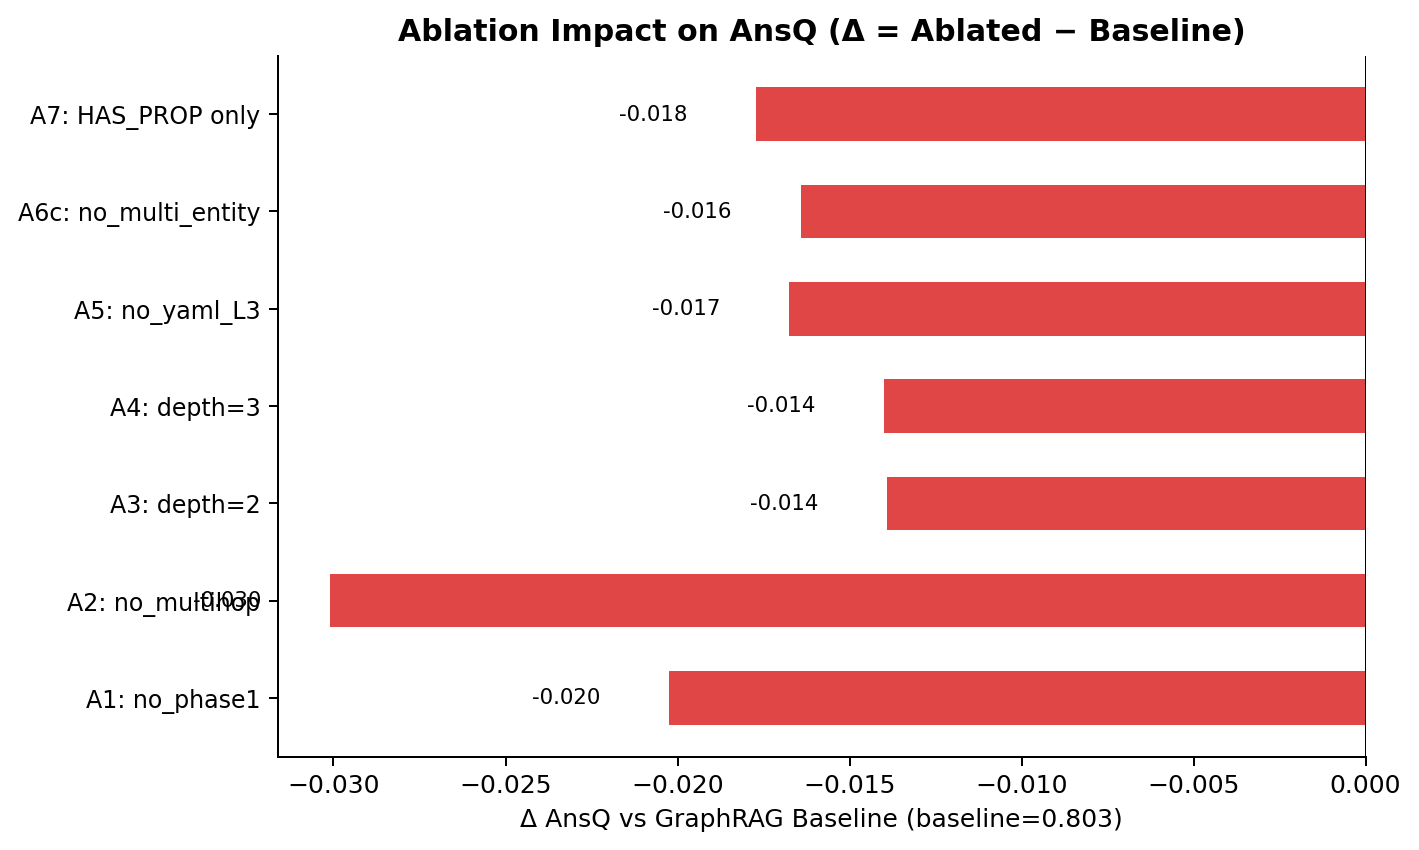
\includegraphics[width=\linewidth]{figures/en/fig2_ablation.png}
    \xfigwd=0pt
    \caption{Drop in RetQ F1 and hop accuracy for each ablation configuration relative to the baseline.}
    \label{fig:ablasi}
\end{figure}

\subsection{Traversal Depth Sensitivity}

Table~\ref{tbl:depth} and Fig.~\ref{fig:depth} report RetQ, AnsQ, and hop accuracy across traversal depths $d \in \{1,\ldots,5\}$, holding every other component fixed at its default configuration.

\begin{table}[t]
\caption{Traversal Depth Sensitivity ($n=102$)}
\label{tbl:depth}
\centering
\begin{tabular}{|c|c|c|c|}
\hline
\textbf{Depth ($d$)} & \textbf{RetQ F1} & \textbf{AnsQ} & \textbf{Hop Accuracy} \\
\hline
1 & 0.3666 & 0.7815 & 0.2574 \\
\hline
2 (default) & \textbf{0.7089} & \textbf{0.8031} & 0.7562 \\
\hline
3 & 0.6593 & 0.7891 & \textbf{0.9007} \\
\hline
4 & 0.6113 & 0.7828 & 0.9007 \\
\hline
5 & 0.5838 & 0.7817 & 0.8760 \\
\hline
\end{tabular}
\\[4pt]
{\footnotesize \raggedright $d=2$ is the adaptive default for the \textit{explain} and \textit{followup} intents; $d=3$ is the adaptive default for \textit{generate\_yaml}, \textit{trace\_relationship}, and \textit{planning}.\par}
\end{table}


A depth of $d=2$, the adaptive default for resource-specific intents, achieves the best joint balance of RetQ (0.71) and AnsQ (0.80). At $d=1$, retrieval is too shallow: RetQ falls sharply to 0.37 because the seed node alone rarely covers the schema dependencies needed to answer the query. Increasing depth beyond 2 improves hop accuracy, which peaks at $d=3$ (0.90), but RetQ declines monotonically thereafter (0.66 at $d=3$, 0.61 at $d=4$, 0.58 at $d=5$) because deeper traversal increasingly draws in the generic, widely shared node types described in \S\ref{sec:perancangan}, diluting precision without adding query-relevant structure. AnsQ is comparatively insensitive to depth once $d\geq2$, ranging narrowly from 0.78 to 0.80, consistent with the finding in \S\ref{sec:hasil}-A that answer quality is governed primarily by the LLM rather than by retrieval. This trade-off between edge recall and retrieval precision is the empirical basis for adapting depth to query intent rather than fixing a single depth for all queries: no single value of $d$ is jointly optimal across RetQ and hop accuracy, and the intents that benefit from deeper traversal (\textit{generate\_yaml}, \textit{trace\_relationship}, and \textit{planning}) are exactly those assigned $d=3$ in this system.

\begin{figure}[t]
    \centering
    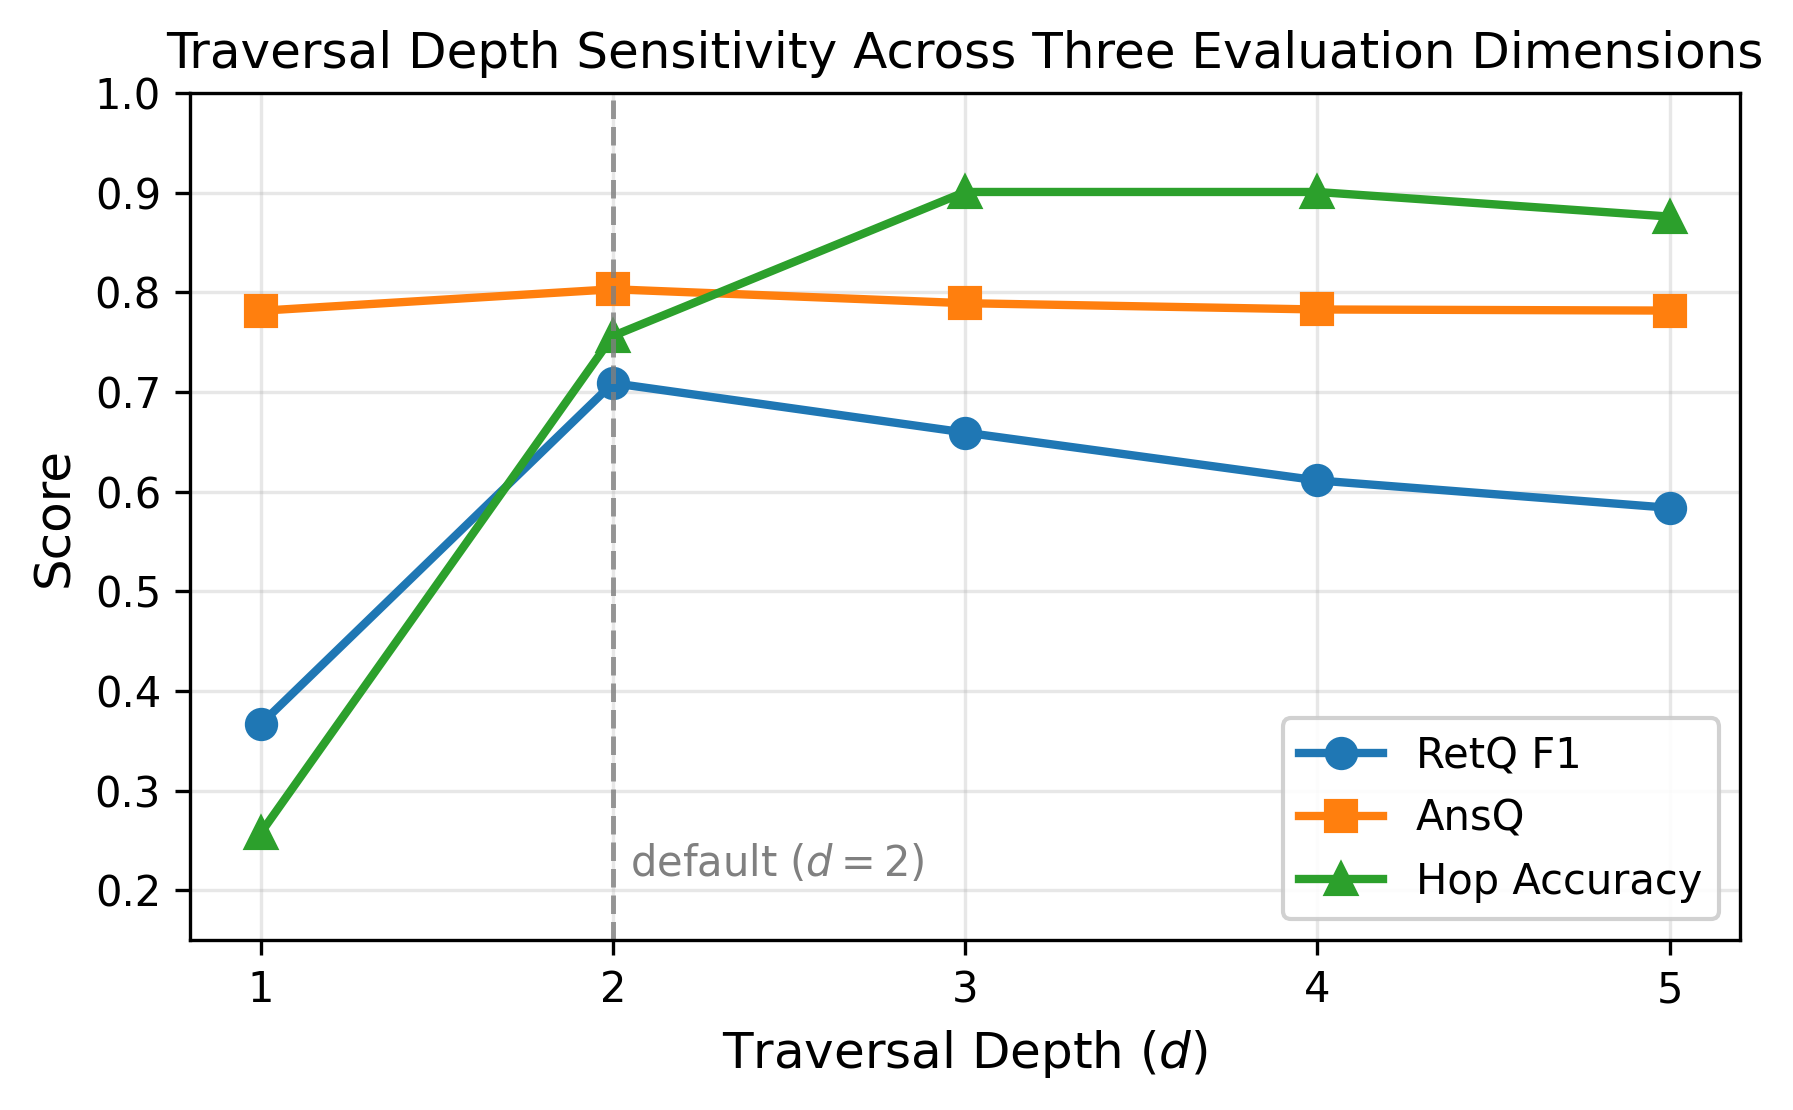
\includegraphics[width=\linewidth]{figures/en/fig3_depth.png}
    \xfigwd=0pt
    \caption{RetQ F1, AnsQ, and hop accuracy as a function of traversal depth $d$.}
    \label{fig:depth}
\end{figure}

\subsection{Boundary Conditions}

To identify where GraphRAG's advantage is largest, Table~\ref{tbl:boundary} reports the mean RetQ gain over Vector RAG for each fixture category, defined as the per-fixture difference in RetQ between the two systems.

\begin{table}[t]
\caption{Mean RetQ Gain over Vector RAG per Fixture Category}
\label{tbl:boundary}
\centering
\begin{tabular}{|l|c|c|}
\hline
\textbf{Category} & \textbf{$n$} & \textbf{Mean Gain} \\
\hline
followup & 12 & \textbf{$+0.6642$} \\
\hline
yaml\_gen & 25 & $+0.5450$ \\
\hline
planning & 5 & $+0.5406$ \\
\hline
command & 3 & $+0.4614$ \\
\hline
troubleshooting & 5 & $+0.4219$ \\
\hline
realworld & 9 & $+0.4014$ \\
\hline
conceptual & 25 & $+0.3870$ \\
\hline
relationship & 18 & $+0.3540$ \\
\hline
\textbf{Overall} & \textbf{102} & \textbf{$+0.467$} \\
\hline
\end{tabular}
\\[4pt]
{\footnotesize \raggedright Spearman correlation between graph node degree and RetQ gain: $\rho=+0.245$, $p=0.013$ ($n=101$), weak but significant. Between hops retrieved and RetQ gain: $\rho=-0.082$, $p=0.414$ ($n=102$), not significant.\par}
\end{table}


GraphRAG outperforms Vector RAG on all eight categories with no exceptions. The gain ranges from $+0.354$ for \textit{relationship} queries, which already state resource relations explicitly and therefore benefit least from additional traversal, to $+0.664$ for \textit{followup} queries, which depend on multi-turn context spanning several resources and therefore benefit most from multi-hop retrieval. The overall mean gain across all 102 fixtures is $+0.467$.

Two structural factors were tested for correlation with this per-fixture gain using Spearman's $\rho$. The degree of the primary node in the knowledge graph (its number of incident edges) correlates weakly but significantly with RetQ gain ($\rho=+0.245$, $p=0.013$, $n=101$): resources with richer schema connectivity, such as \textit{Deployment} and \textit{StatefulSet}, benefit more from multi-hop traversal because more relevant context becomes reachable. In contrast, the number of hops actually retrieved during evaluation shows no significant correlation with gain ($\rho=-0.082$, $p=0.414$), indicating that traversal depth per fixture is not by itself a strong predictor of GraphRAG's advantage; the advantage instead depends on the structural richness of the resource being queried.

\subsection{Discussion: Faithfulness and the Limits of the Advantage}

GraphRAG's faithfulness (0.31) is significantly higher than Vector RAG's (0.17), yet its absolute value remains well below an ideal threshold. To quantify this gap, all 818 claims extracted from GraphRAG's answers across the full fixture set were classified into four categories: \textit{supported} (258 claims, 31.5\%, directly traceable to the retrieved graph context), \textit{modality} (81 claims, 9.9\%, content supported by the context but reformulated from a declarative schema statement into a procedural instruction), \textit{partial} (24 claims, 2.9\%, combining a context-supported component with LLM-added detail), and \textit{absent} (455 claims, 55.6\%, with no traceable reference in the retrieved context). Combining the first two categories, only 41.4\% of claims (339 of 818) are traceable to document context, while the majority originate from the LLM's parametric knowledge rather than from the retrieved graph.

This is not a system defect but an architectural consequence: the knowledge graph, built from the \textit{definitions} block, only models object-typed inter-resource relations as edges, while scalar attribute values (such as a container name or image) cannot be represented as graph nodes. The system is therefore deliberately designed to be open-book: the LLM is allowed to complete its answer with parametric knowledge when information is unavailable in the graph. Correlation analysis shows that faithfulness correlates weakly and non-significantly with AnsQ, confirming that the two measure different things: AnsQ measures answer correctness and relevance, while faithfulness measures the traceability of claims to the retrieved context.

\subsection{Limitations}

Three limitations further bound the scope of these findings. First, the knowledge graph built is static and represents only schema-structural relations from the \textit{definitions} block; operational relations such as RBAC bindings are reachable in only one direction, and live cluster runtime state is not represented. Second, retrieval is capped at three hops, so queries requiring context beyond this reach silently fall back on the LLM's parametric knowledge. Among all categories, the \textit{relationship} category receives the smallest, though still positive, benefit from GraphRAG. Third, GraphRAG's advantage does not extend to every evaluation dimension: AnsQ is on par with Vector RAG, and faithfulness reflects the graph's limited coverage of attribute values rather than a failure of the retrieval mechanism itself.

\section{Conclusion}
\label{sec:kesimpulan}

This work builds a GraphRAG system with three technical contributions: deterministic knowledge-graph construction from the Kubernetes OpenAPI schema, a retrieval mechanism with traversal depth adapted per query intent, and three-layer, graph-grounded YAML validation as an alternative to a live-cluster dry-run. Evaluation on 102 test scenarios shows a significant GraphRAG advantage in retrieval (F1 0.71 versus 0.24, $\Delta{+}0.465$ over Vector RAG) and structural reasoning, while answer quality remains comparable across systems since it depends on the same underlying LLM. These findings confirm that graph representation's contribution in the Kubernetes configuration domain lies in the traceability and completeness of structural retrieval, not in answer fluency.

\section*{Acknowledgment}
This manuscript was prepared with LLM assistance to condense text from the first author's undergraduate thesis; all technical claims, data, and experimental results originate from research conducted and validated by the authors.

\bibliographystyle{IEEEtran}
\bibliography{refs}

\begin{biography}[{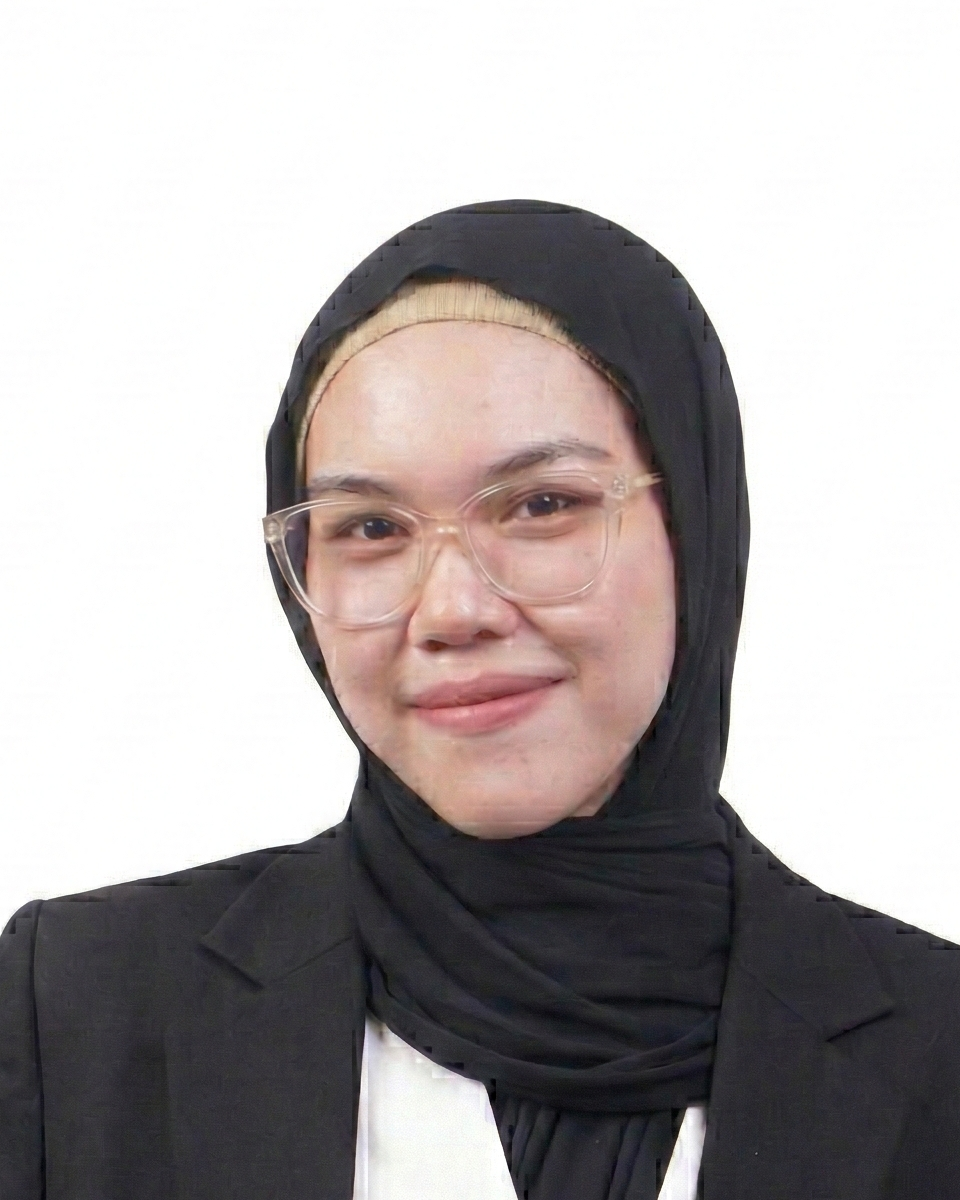
\includegraphics[width=1in,height=1.25in,clip,keepaspectratio]{figures/en/profile_bio.png}}]{Jihan Aurelia}
is pursuing her bachelor's degree in Information Systems and Technology at the School of Electrical Engineering and Informatics, Institut Teknologi Bandung, Indonesia. Her undergraduate thesis develops a graph-based retrieval-augmented generation system for Kubernetes configuration. Her research interests include knowledge graph construction and retrieval-augmented generation for large language models.\EOD
\end{biography}

\end{document}
